\newpage 
\section{A new machine learning-based recommender system for context-based emotion regulation strategy recommendation}~\label{sec:evaluation}
Digital technologies are increasingly being used to implement psychological interventions due to their high efficiency and scalability. More people than ever have access to a variety of affordable technologies due to digital technologies' connectivity, mobility, and multifunctionality, and owing to how easily users can navigate through apps, they can participate in digital emotion regulation \cite{reynarddigital}, \cite{bettis2022digital}. Digital technologies offer a promising approach to improve ER delivery to a group or individual intervention. Although it is clear that digital technology offers a wide range of opportunities for interventions in emotion regulation, the adoption of such a delivery method is currently hindered by significant challenges for example, digital literacy, effective digital communication, and online well-being \cite{jadhakhan2022efficacy}. As previously stated in the literature, online toxicity may be caused by ineffective emotion regulation; therefore, technological interventions aimed at supporting ER should also aim to improve online well-being.

Supporting DER necessitates first considering the structure of the designed intervention in the context of the delivery mechanisms that digital technology can introduce into the intervention process: i.e., how, when, and where the design is supposed to scaffold participants' learning. The first challenge is that learning to be aware of, attentive to, and capable of modifying various physiological processes is emphasised in the development of ER skills. Because these processes are internal body states that are difficult to perceive, articulate, and directly observe in an online application, real-time, accurate external feedback is difficult and highly subjective \cite{slovak2022designing}, \cite{tag2022emotion}. Another challenge is the lack of assistance for users to apply newly acquired skills in daily life. The vast majority of interaction design research focuses on physiological synchronisation or providing users with external input that mimics their biosignals, such as false heart rate, reminders and recommendations of specific ER strategies, and awareness systems that support monitoring and/or tracking of individual emotions. Outside of its effects on technology use, these methods undervalue the importance of intervention transfer. They believe that for the intervention to be effective, the developed systems must provide ongoing support and that removing a system such as wearable feedback would render the effects ineffective. A few interventions designed to help children and adolescents with anxiety and self-regulation learning, as well as reduce application dependence over time, do not provide on-the-spot support \cite{antle2018opening}, \cite{antle2019design}, \cite{scholten2016randomized}, \cite{slovak2016scaffolding}. As a result, the goal of this study is to embed didactic ER learning as a transferable skill by providing on-the-spot support in the form of context-based recommendations for ER strategies. Because the framework from the first research question is based on both content and context, we intend to use this broader context to fuel ER recommendations rather than appraisal or suppression of emotions. Therefore, in this research we try to answer the following research questions:
\begin{itemize}
    \item What factors constitute the context for recommending an ER strategy when providing on-the-spot emotion regulation support?
    \item How can support for Emotion Regulation be expanded to include a variety of ER strategies rather than just suppression and reappraisal in all contexts?
    \item How can information delivery in online ER recommendation environments be customised for users and presented as a transferable skill?
\end{itemize}
\begin{figure}[h]
  
    \centering
    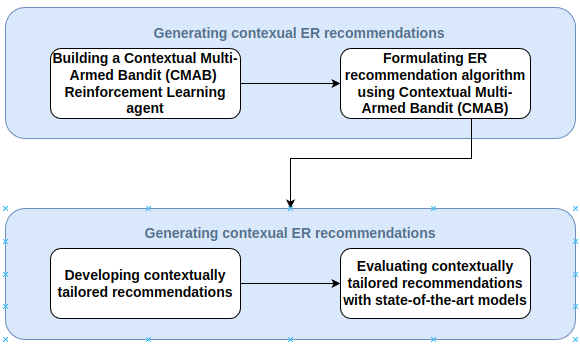
\includegraphics[width=12cm,height=12cm,keepaspectratio]{res3.png}
%   \includegraphics[width=5cm,height=5cm,keepaspectratio]{samples/sample_convv.png}
%   \includegraphics[width=5cm,height=5cm,keepaspectratio]{samples/sample_conv_graphh.png}
  \caption{Proposed methodology for calculating the effect of an induced emotion on a conversation}
  \label{fig:Frameworkres3}
  \end{figure} 
\subsection{Proposed methodology}~\label{subsec:RQs}
Since the need to regulate emotions here has been identified based on the need to regulate the emotions expressed in a conversation, recommendations for appropriate ER strategies need to be fuelled by (psychological) theory-backed inputs, context as well as user preferences. Given the limited number of ER strategies, it is essential for the recommendation system to be able to adapt to the dynamic nature of online conversations to extract context and provide real-world decision-making aid for the users.
\begin{itemize}
    \item The first step involves formulating emotion regulation recommendation algorithm using contextual multi-armed bandits. Contextual multi-armed bandit (CMAB) is a reinforcement learning algorithm that makes use of contextual data to learn a policy that initiates actions depending on the context in order to maximise expected rewards. CMABs have been used successfully in the development of mobile-health interventions for ER \cite{beltzer2022building}, \cite{ameko2020offline}. This model would be able to recommend ER strategies to users by capturing the current state of a conversation.
    \item Because cognitive appraisal or suppression is the most common ER strategy suggested by ER interventions \cite{aldao2010emotion}, we plan to compare the number of instances where the model suggests these two strategies, as we believe contextually tailored recommendations must be more effective than using cognitive reappraisal indiscriminately across all contexts. This experiment's proposed methodology is shown in Figure-\ref{fig:Frameworkres3}
\end{itemize}